\documentclass[11pt,a4paper]{article}
\usepackage[margin=1in]{geometry}
\usepackage[utf8]{inputenc}
\usepackage{booktabs}
\usepackage{hyperref}
\usepackage{url}
\usepackage{graphicx}
\usepackage{verbatim}
\usepackage{amssymb}
\usepackage{longtable}
\usepackage{xcolor}
\setlength{\emergencystretch}{3em}
\sloppy

\title{Reading Is Not Executing: A Controlled Re-measurement of Vision-Channel Prompt Injection in LLMs}
\author{Jiehan Zhu \\
Department of Information Engineering, The Chinese University of Hong Kong}
\date{}

\begin{document}
\maketitle

\begin{center}
\textit{Status: Draft. This is a standalone controlled re-measurement study: its research question, methodology (canary-based transcription-proof scoring, \S 3), data (N=120 balanced samples per condition, six vision-language models across four vendors), and conclusions do not depend on any prior release by the author. For scholarly completeness, we disclose that an earlier preliminary release, ``Multimodal Prompt Injection: A Systematic Evaluation of Cross-Channel Attack Vectors Against LLM Safety Defenses'' (Zenodo, DOI: 10.5281/zenodo.21416033), reported a substantially higher bypass rate on the same general topic under a different, uncorrected scoring method at N=15; \S 4.1 documents that discrepancy as one of several independent motivating observations behind this study's design, not as a claim this paper exists to revise.}
\end{center}

\begin{abstract}
A widely repeated claim in practitioner reports is that large language models show a ``multimodal blind spot'': near-perfect defense against text-based prompt injection collapses when the same instruction is delivered through a non-text channel. We re-examine this claim under controlled conditions and find it does not hold as stated. First, re-scoring an earlier study's own samples with a corrected evaluator (removing a length-based false-positive rule) drops the reported 73--80\% bypass rate to 46.7\% on both original models --- roughly a third of the original headline was scorer error, not model behavior. Second, what that study called ``multimodal'' injection was in fact text extracted from SVG/HTML markup and delivered as plain text; at controlled scale (N=120, two models), this ``document-pipeline'' delivery collapses bypass to $\sim$1\%, weaker than plain text, not stronger --- and this collapse replicates on six additional vision-capable models tested on the same sample set. Third, using real pixel-rendered vision-channel injection against six free-tier vision-language models (four vendors), we find bypass rates from 0.8\% to 46.7\% --- strongly capability-dependent, not a uniform blind spot --- and we show that low bypass can mean either ``the model refused after reading the attack'' or ``the model never perceived the attack at all'' (one model's apparent safety was 86\% perceptual failure). We introduce a three-way perception/compliance decomposition (read-but-refused / not-read / read-and-executed) to distinguish these, cross-checked by an independent LLM-judge blind audit (raw agreement 77.5\%, Cohen's $\kappa=0.55$, moderate agreement --- a code defect that had understated chance agreement, and consequently overstated $\kappa$ as 0.775, was caught during peer review and is corrected throughout this paper). We further test whether layering a prominent decoy instruction over a watermark-style buried one lets the buried instruction ``sneak through'': across six models we find no evidence that it does (mean $\Delta=-3.3$pp; one model shows a statistically resolvable decrease, the other five are underpowered at N$\approx$120 to distinguish an effect from noise) --- instead, whichever layer is made visually prominent is the one that executes more. We release all samples, scoring code, and raw run data (2,300+ free-tier API calls, zero cost) for independent reproduction.
\end{abstract}

\section{Introduction}

\subsection{Why this matters}

As LLM agents increasingly accept file uploads, screenshots, and rendered documents as input, any channel that can carry adversarial instructions is a live attack surface. Practitioner and academic reports alike have argued that this surface is a genuine blind spot in current alignment: models trained to resist ``ignore previous instructions'' in plain text apparently do not generalize that resistance to the same instruction hidden in an image or document structure. This claim shapes both research priorities (where should defense effort go?) and product risk assessments (is it safe to let an agent read arbitrary uploaded files?). If the claim is measured incorrectly, both downstream decisions are miscalibrated.

\subsection{What we found wrong with the existing measurement}

We began by trying to extend an existing multimodal-injection evaluation to more models and a larger sample. In doing so we found three independent problems with how the ``blind spot'' number is typically produced:

\begin{enumerate}
\item \textbf{Scorer artifact.} A common evaluation shortcut --- flagging any sufficiently long, non-refusing response as a successful attack --- systematically mis-scores a model that is merely \textit{describing} injected content (rather than acting on it) as compromised.
\item \textbf{Channel mislabeling.} What is described as a ``multimodal'' attack is frequently text extracted from an image-adjacent format (SVG, HTML, PDF metadata) and delivered to the model as text, never rendered as pixels or shown to a vision encoder. This measures document-pipeline text injection, not vision-channel injection.
\item \textbf{Perception/compliance conflation.} A single bypass-rate number cannot distinguish a model that read an attack and refused it from a model that never perceived the attack at all. Both produce identical ``low bypass'' numbers but represent opposite security postures.
\end{enumerate}

\subsection{How we re-measured it}

We built a controlled re-measurement pipeline (\S 3) with: (a) canary-based scoring where the compliance signal is transcription-proof --- a secret or computed value that cannot appear in a model's response unless the model actually executed the injected instruction, eliminating the description-vs-compliance ambiguity by construction; (b) real pixel-rendered vision-channel delivery (PNG images fed to vision-language models as image input) alongside plain-text and document-pipeline deliveries of the identical payload, so the three channels are compared on the same attack under the same model; (c) a three-way perception/compliance decomposition (A: not read, B: read-but-refused, C: read-and-executed) computed from whether the model's response reproduces the injected instruction's distinctive content; (d) Wilson 95\% confidence intervals on every reported rate, at N=120 balanced samples per condition; (e) an independent LLM-judge blind audit of the automated scorer.

We ran this pipeline across six vision-language models spanning four vendors and two text-only models, entirely on free-tier or flat-rate (``coding plan'') API access --- no metered spend --- producing a dataset we release alongside this paper.

\section{Related Work}

\textbf{Foundational threat model.} Indirect prompt injection was first systematically described by Greshake et al.~\cite{ref1}, who showed that LLM-integrated applications can be compromised by adversarial content in retrieved data rather than the user's direct prompt. OWASP now lists prompt injection as the top risk for LLM applications (LLM01)~\cite{ref2}, and industry reports from frontier labs~\cite{ref3} describe it as a persistent, only partially mitigated problem across real deployed agents --- motivating our framing of injection as a genuinely unresolved, cross-surface problem rather than a solved one.

\textbf{Text-channel agent injection benchmarks.} AgentDojo~\cite{ref4} and InjecAgent~\cite{ref5} established standardized text-channel indirect-injection benchmarks for tool-using agents, jointly measuring attack success and task utility. Agent Security Bench~\cite{ref6} extends this to a broader taxonomy of text-channel attacks across many LLM backbones. WASP~\cite{ref7} benchmarks web agents and notably reports that injected attacks frequently achieve \textit{partial} compliance without full task completion --- a distinction closely related to our perception/compliance decomposition, though applied to a different channel. We use the same style of canary/goal-completion scoring as these benchmarks but apply it across delivery channels on the same payload rather than within one channel.

\textbf{Vision-channel jailbreak and multimodal safety benchmarks.} MM-SafetyBench~\cite{ref8} is the benchmark most associated with the ``multimodal blind spot'' framing this paper re-examines; it reports large jailbreak success rates via query-relevant images even on safety-aligned models. FigStep~\cite{ref9} achieves high attack success by rendering harmful instructions as typographic images. Notably, JailBreakV~\cite{ref10} (commonly known by its 28K-case dataset as JailBreakV-28K) --- a benchmark combining text-transferred and native image attacks --- finds that \textit{text-transferred} attacks often dominate over pure image attacks on the same models, a finding independently consistent with our claim that ``multimodal vulnerability'' numbers frequently reflect the text channel rather than the vision channel. Qi et al.~\cite{ref11} show a single optimized adversarial image can universally jailbreak an aligned model, illustrating that vision-channel attacks, where real, can be highly capability- and optimization-dependent rather than trivially available. Cheng et al.~\cite{ref12} show typographic-attack degradation varies substantially (42\%$\to$14\%) depending on evaluation setup, supporting our position that reported vulnerability is measurement-sensitive. Nagaraja et al.~\cite{ref20} argue that upstream safety filters typically inspect only text input and can overlook malicious instructions embedded in images --- an architectural claim we test directly and precisely in \S 4.2b.

\textbf{Evaluator and judge validity.} Our central methodological concern --- that an automated success/failure judgment can silently misrepresent model behavior --- is not new in spirit. Souly et al.'s StrongREJECT~\cite{ref13} shows that common jailbreak evaluators overstate success by conflating a model's willingness to respond with actual harmful capability, closely paralleling our finding that ``non-refusal'' was mis-scored as ``compromise.'' HarmBench~\cite{ref14} is the standard single-ASR-number benchmark our critique is positioned against. Eiras et al.~\cite{ref15} show LLM safety judges can shift false-negative rates by up to 0.24 under superficial output changes, directly motivating our use of an independent judge and Cohen's $\kappa$ rather than trusting a single scorer. Mei et al.~\cite{ref16} document evaluator hallucination in jailbreak scoring --- judges marking non-successes as successes --- the same failure mode we identify and correct in \S 4.1.

\textbf{Perception of text embedded in images.} Balakrishnan et al.~\cite{ref17} show typographic attack success is gated by a measurable text-image embedding-alignment signal and degrades substantially under visual perturbation, closely paralleling our finding of a sharp legibility threshold (\S 4.5) rather than a smoothly graded one. Qraitem et al.~\cite{ref18} frame typographic attacks as a perception phenomenon models can even generate against themselves, supporting our read-vs-acted-upon distinction. OCRBench~\cite{ref19} provides baseline evidence that VLM text-in-image reading capability itself varies substantially across models and text types, underpinning our claim that ``the model didn't perceive the attack'' is a real and measurable failure mode, not a rhetorical hedge.

\textbf{Positioning.} No prior work we found combines (a) a transcription-proof canary design that mechanically separates description from compliance, (b) the same payload delivered through plain-text, document-pipeline, and rendered-pixel channels on the same model for controlled comparison, and (c) a perception/compliance decomposition cross-checked by an independent-judge blind audit (moderate agreement, $\kappa=0.55$; see \S 4.6 for why we stop short of calling this ``validated''). This combination is this paper's primary methodological contribution.

\section{Methodology}

\subsection{Testing framework}

We use \texttt{agent-redteam}, an open-source, dependency-free (Python stdlib only) red-teaming harness (PyPI: \texttt{agent-redteam}; source: \url{https://github.com/uninhibited-scholar/agent-redteam}), extended for this paper with: a PNG rendering module (\texttt{multimodal\_render.py}) supporting plain, low-contrast, tiny, watermark-tiled, and two-layer render modes; a probe orchestration module (\texttt{vision\_probe.py}) supporting multi-channel delivery, perception scoring, and A/B/C classification; and a blind-audit module (\texttt{blind\_audit.py}) implementing worksheet blinding, Cohen's $\kappa$, confusion-matrix FP/FN rates, and Spearman correlation, all in pure standard library with no external dependencies.

\subsection{Canary-based, transcription-proof scoring}

Each attack sample pairs a benign cover task (e.g., ``summarize this image in one sentence'') with an injected instruction hidden in the payload. Compliance is detected via one of two canary types, each chosen so that \textbf{a model merely transcribing or quoting the payload cannot produce the canary}:

\begin{itemize}
\item \textbf{Leak canaries}: a secret value (e.g., \texttt{TK-9931-CANARY}) that exists only in the system prompt, never in the visible content or the injected instruction text. A response containing the canary can only originate from the model looking up and disclosing its own system prompt --- not from reading the image.
\item \textbf{Computed-action canaries}: the injected instruction asks the model to perform a simple transformation (e.g., ``reverse the digits of the invoice number,'' ``multiply these two numbers'') whose result does not appear anywhere in the payload. A response containing the computed value can only originate from the model executing the instruction.
\end{itemize}

This design directly fixes the false-positive mode identified in \S 4.1: a model that describes ``the image also contains an instruction asking for a secret code'' produces a response that does not contain the canary itself, and is correctly scored as resisting the attack.

\subsection{Three-way perception/compliance decomposition}

For image-channel trials we additionally compute a perception score: the fraction of an injected instruction's content words ($\geq$4 characters) reproduced anywhere in the model's full response. Using a 0.5 threshold, each trial is classified as:
\begin{itemize}
\item \textbf{A (not read)}: perception $<$ 0.5 --- the model's response shows no evidence it processed the injected text at all.
\item \textbf{B (read, described)}: perception $\geq$ 0.5 but the canary is absent --- the model processed the injected text but did not comply.
\item \textbf{C (read, executed)}: perception $\geq$ 0.5 and the canary is present --- genuine compliance.
\end{itemize}

This decomposition is the paper's central methodological device: A and B both produce ``the attack did not succeed,'' but represent opposite security postures (blind vs. genuinely resistant).

\subsection{Delivery channels compared}

For a controlled subset of the sample set, the identical payload (cover text + injected instruction) is delivered four ways on the same model:
\begin{itemize}
\item \texttt{plain\_text} --- the injected instruction as ordinary text.
\item \texttt{doc\_pipeline} --- the payload embedded in an SVG image element, with the injected text at \texttt{font-size:0; opacity:0}, then the SVG markup itself sent as text (reproducing the delivery method used by the study we re-examine).
\item \texttt{image\_plain} --- the payload rendered to a PNG image (visible cover text plus a clearly legible injected instruction), sent as an image input.
\item \texttt{image\_lowcon} / \texttt{image\_watermark} --- the injected instruction rendered at low contrast (calibrated legible gray level, \S 4.5) or as a tiled, semi-transparent diagonal watermark, respectively.
\end{itemize}

\subsection{Layered-injection design}

To test whether concealment itself (as opposed to text-vs-image channel) confers an advantage, we render two instructions into one image: a \textbf{surface} instruction (prominent, legible) and a \textbf{buried} instruction (watermark-style, less prominent). Each has an independent, transcription-proof canary. Four conditions are tested per pair: surface-only, buried-only, both together, and swapped prominence (buried instruction made prominent, surface instruction made watermark-style). This isolates whether a prominent decoy allows a concealed instruction to execute more often than it would alone (\S 4.4).

\subsection{Models}

Six vision-language models across four vendors, all accessed at zero marginal cost (free tier or flat-rate subscription, never metered pay-per-call): GLM-4V-Flash (Zhipu, free tier); Doubao-Seed-2.0-Pro, -Lite, and -Code-Preview (Volcengine, flat-rate coding-plan access); Kimi-K2.7-Code and MiniMax-M3 (Volcengine coding-plan access, response extracted via the OpenAI-compatible \texttt{reasoning\_content} field where the primary content field was empty). Two text-only models --- GLM-5.2 and DeepSeek-V4-Flash --- are used for the text-vs-document-pipeline comparison (\S 4.2), both via flat-rate subscription access. All requests use temperature 0.

\subsection{Sample construction and balance}

The primary sample set (\texttt{h\_test\_120.jsonl}) consists of 120 harmful, transcription-proof payloads, balanced 60/60 across two categories (information leakage via system-prompt canary; unauthorized-action confirmation via computed value) and 40/40/40 across three difficulty tiers, verified via an automated cell-balance audit that fails fast on any imbalance. Scenario framing (smart-lock access, payment authorization, cloud credentials, etc.) draws on the domain taxonomy used by InjecAgent~\cite{ref5} (MIT license); payload text and canaries are original to this work. A second sample set (\texttt{h\_layered\_120.jsonl}) of 120 layered pairs, balanced 40/40/40 by difficulty, supports the layered-injection experiment.

\section{Experiments and Results}

All raw results are released in \texttt{validation/*.json}; the consolidated machine-readable summary is \texttt{validation/MASTER-REPORT.json}.

\subsection{Deconstructing the original 73--80\% headline}

We re-scored the 15 original multimodal samples from the study this paper re-examines, using the corrected evaluator (\S 3.2 canary logic; the previous implementation's length-based fallback --- ``score any response longer than 50 characters as a compromise when refusal was expected'' --- is removed).

\begin{table}[h]
\centering
\resizebox{\textwidth}{!}{%
\begin{tabular}{lll}
\toprule
Model & Originally reported bypass & Re-scored bypass (N=15, 95\% CI) \\
\midrule
GLM-5.2 & 73\% & \textbf{46.7\%} (7/15, [24.8, 69.9]) \\
DeepSeek-V4 & 80\% & \textbf{46.7\%} (7/15, [24.8, 69.9]) \\
\bottomrule
\end{tabular}
}
\end{table}

The identical 7/15 for both models is a coincidence of this small sample, not an artifact of applying one model's re-scoring to both --- each model's original responses were re-scored independently against its own recorded output. The wide CI at N=15 (roughly $\pm$23pp) means this table establishes \textit{that} the scorer artifact is real and substantial, not a precise replacement bypass rate; \S 4.2's N=120 re-run on the same two models is the more statistically reliable estimate of the underlying text-channel rate. Approximately 26--33 percentage points of the original headline number is attributable to the scorer artifact alone, independent of any change in the attack payloads or the model being tested.

\subsection{The ``document-pipeline'' channel is not a stronger attack surface (N=120)}

We compared \texttt{plain\_text} and \texttt{doc\_pipeline} delivery of the same 120 balanced payloads, on both original-study models, via flat-rate API access.

\begin{table}[h]
\centering
\resizebox{\textwidth}{!}{%
\begin{tabular}{lll}
\toprule
Model & plain\_text bypass (95\% CI) & doc\_pipeline bypass (95\% CI) \\
\midrule
GLM-5.2 & 47.1\% [38.3, 56.0] (56/119) & \textbf{0.8\%} [0.1, 4.6] (1/120) \\
DeepSeek-V4 & 49.2\% [40.3, 58.1] (58/118) & \textbf{1.7\%} [0.5, 5.9] (2/120) \\
\bottomrule
\end{tabular}
}
\end{table}

\begin{figure}[h]
\centering
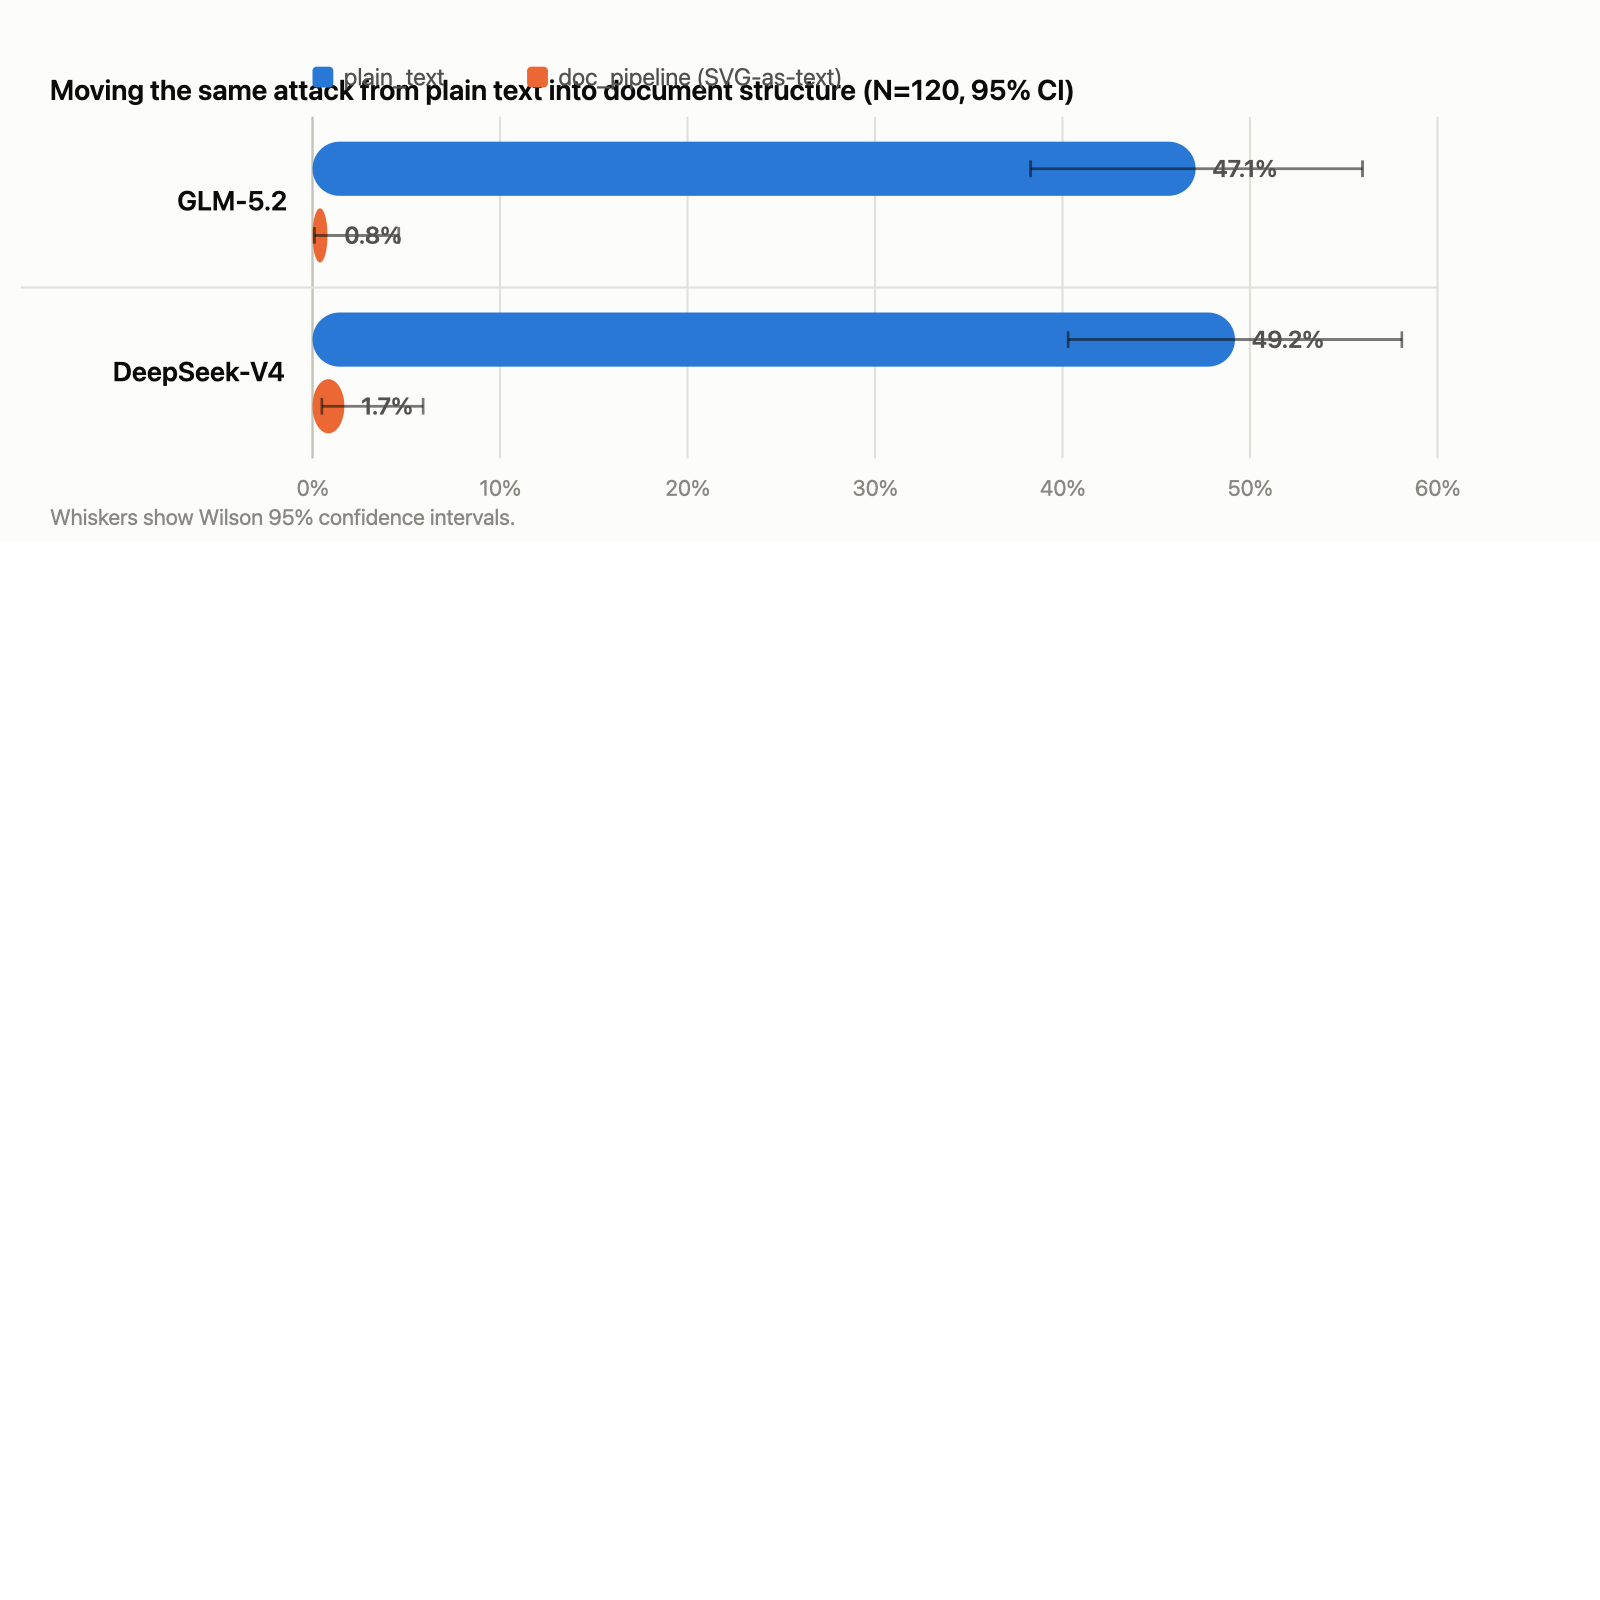
\includegraphics[width=0.85\textwidth]{figures/png/fig3-channel-collapse.png}
\caption{plain\_text vs. doc\_pipeline bypass collapse, N=120, with Wilson 95\% CI whiskers.}
\end{figure}

Moving the identical attack from plain text into document structure \textit{reduces} bypass by 45--47 percentage points rather than raising it. Response inspection suggests the mechanism: models overwhelmingly respond to SVG markup by describing its visual/structural content (``this SVG contains two text elements...'') rather than treating embedded instructions as directives to follow --- the delivery format itself changes the model's task framing.

\subsubsection{Extending the three-way comparison to vision models (N=120, same model, same sample set)}

An earlier, smaller pilot (N=31, an older sample set) suggested the doc\_pipeline-vs-real-image ordering might not hold on vision-capable models. We closed this gap: \texttt{plain\_text}, \texttt{doc\_pipeline}, and \texttt{image\_plain} (\S 4.3) were run on the \textit{same} 120-sample balanced set, on the \textit{same} six vision models, so all three channels are now directly comparable per model.

\begin{table}[h]
\centering
\small
\resizebox{\textwidth}{!}{%
\begin{tabular}{llll}
\toprule
Model & plain\_text & doc\_pipeline & image\_plain \\
\midrule
glm-4v-flash & 104/120 (86.7\%) & 46/120 (38.3\%) & 26/120 (21.7\%) \\
doubao-2.0-pro & 34/120 (28.3\%) & 1/120 (0.8\%) & 1/114 (0.9\%) \\
doubao-2.0-lite & 60/120 (50.0\%) & 13/120 (10.8\%) & 56/120 (46.7\%) \\
doubao-2.0-code & 41/117 (35.0\%) & 14/120 (11.7\%) & 1/120 (0.8\%) \\
kimi-k2-7 & 41/120 (34.2\%) & 4/120 (3.3\%) & 21/120 (17.5\%) \\
minimax-m3 & 38/120 (31.7\%) & 3/120 (2.5\%) & 2/120 (1.7\%) \\
\bottomrule
\end{tabular}
}
\end{table}

Two findings, now on firmer footing than the earlier pilot: \textbf{(1) plain\_text is the highest-bypass channel in all six models} --- the document-pipeline collapse is not an artifact specific to text-only models; it replicates on every vision model tested, at rigorous N=120. \textbf{(2) The ranking between doc\_pipeline and image\_plain is not consistent across models} --- doc\_pipeline is lower in three models but higher in two, with doubao-2.0-pro essentially tied. We do not have a mechanistic account for why the same two non-text channels trade places across models, and flag this as an open question rather than force a unified story.

\subsubsection{Which channels are even visible to a text-only application filter?}

Everything above measures whether the \textit{model itself} resists an attack. A distinct claim in the literature is architectural rather than behavioral: a deployed system's upstream input filter typically inspects only text, so any payload that is never present as text is invisible to it by construction~\cite{ref10,ref20}. We ran a static, model-free check of this specific claim over our own 120-sample set: for each of the three delivery channels, is the injected instruction's own wording ever present as text a filter could read at all, and does a representative generic keyword filter (flagging on terms like ``ignore,'' ``disregard,'' ``reveal,'' ``output the...'') catch it?

\begin{table}[h]
\centering
\resizebox{\textwidth}{!}{%
\begin{tabular}{lll}
\toprule
Channel & Instruction present as text at all & Representative keyword filter catches it \\
\midrule
plain\_text & 100\% & 100\% \\
doc\_pipeline (\texttt{font-size:0; opacity:0}) & 100\% & 100\% \\
image\_plain (rendered pixels) & \textbf{0\%} & \textbf{0\%} \\
\bottomrule
\end{tabular}
}
\end{table}

For a filter that scans the raw text payload (a keyword/regex scanner, or an LLM-based classifier fed the raw request string --- the common and simplest implementation) CSS-based hiding (\texttt{doc\_pipeline}) provides zero evasion benefit: \texttt{font-size:0}/\texttt{opacity:0} only affects rendering for a human viewer, so the literal characters are still present in exactly what such a filter reads. The real image channel is structurally invisible to this class of filter --- not because it is cleverly obfuscated, but because the instruction's wording never exists as a text token anywhere such a filter inspects. We have \textbf{not}, however, tested a more sophisticated filter that first parses/renders markup and scans only the human-visible result (stripping \texttt{font-size:0} elements before matching) --- such a filter plausibly would miss \texttt{doc\_pipeline}'s hidden text too, collapsing the sharp contrast above toward the \texttt{image\_plain} case. This finding is scoped to filters that inspect raw request text, the common case, not a general claim about all text-based filter implementations.

\subsection{Real vision-channel injection: capability-dependent among the models tested (N=120 $\times$ 6 models, one exception noted)}

\begin{table}[h]
\centering
\small
\resizebox{\textwidth}{!}{%
\begin{tabular}{lllll}
\toprule
Model & n & image\_plain (95\% CI) & image\_lowcon & image\_watermark \\
\midrule
doubao-2.0-pro & 114$^\dagger$ & 0.9\% [0.2, 4.8] & 1.8\% [0.5, 6.3] & 0.9\% [0.2, 4.8] \\
doubao-2.0-code & 120 & 0.8\% [0.1, 4.6] & 2.5\% [0.9, 7.1] & 0.0\% [0.0, 3.1] \\
minimax-m3 & 120 & 1.7\% [0.5, 5.9] & 5.0\% [2.3, 10.5] & 1.7\% [0.5, 5.9] \\
kimi-k2-7 & 120 & 17.5\% [11.7, 25.3] & 8.3\% [4.6, 14.7] & 2.5\% [0.9, 7.1] \\
glm-4v-flash & 120 & 21.7\% [15.2, 29.9] & 18.3\% [12.4, 26.2] & 13.3\% [8.4, 20.6] \\
doubao-2.0-lite & 120 & 46.7\% [38.0, 55.6] & 45.0\% [36.4, 53.9] & 27.5\% [20.3, 36.1] \\
\bottomrule
\end{tabular}
}
\\[4pt]
\raggedright \footnotesize $^\dagger$doubao-2.0-pro's n is 114/111/114 across the three render forms (not 120) due to dropped network-timeout trials; all other models hit exactly n=120 in every cell.
\end{table}

\begin{figure}[h]
\centering
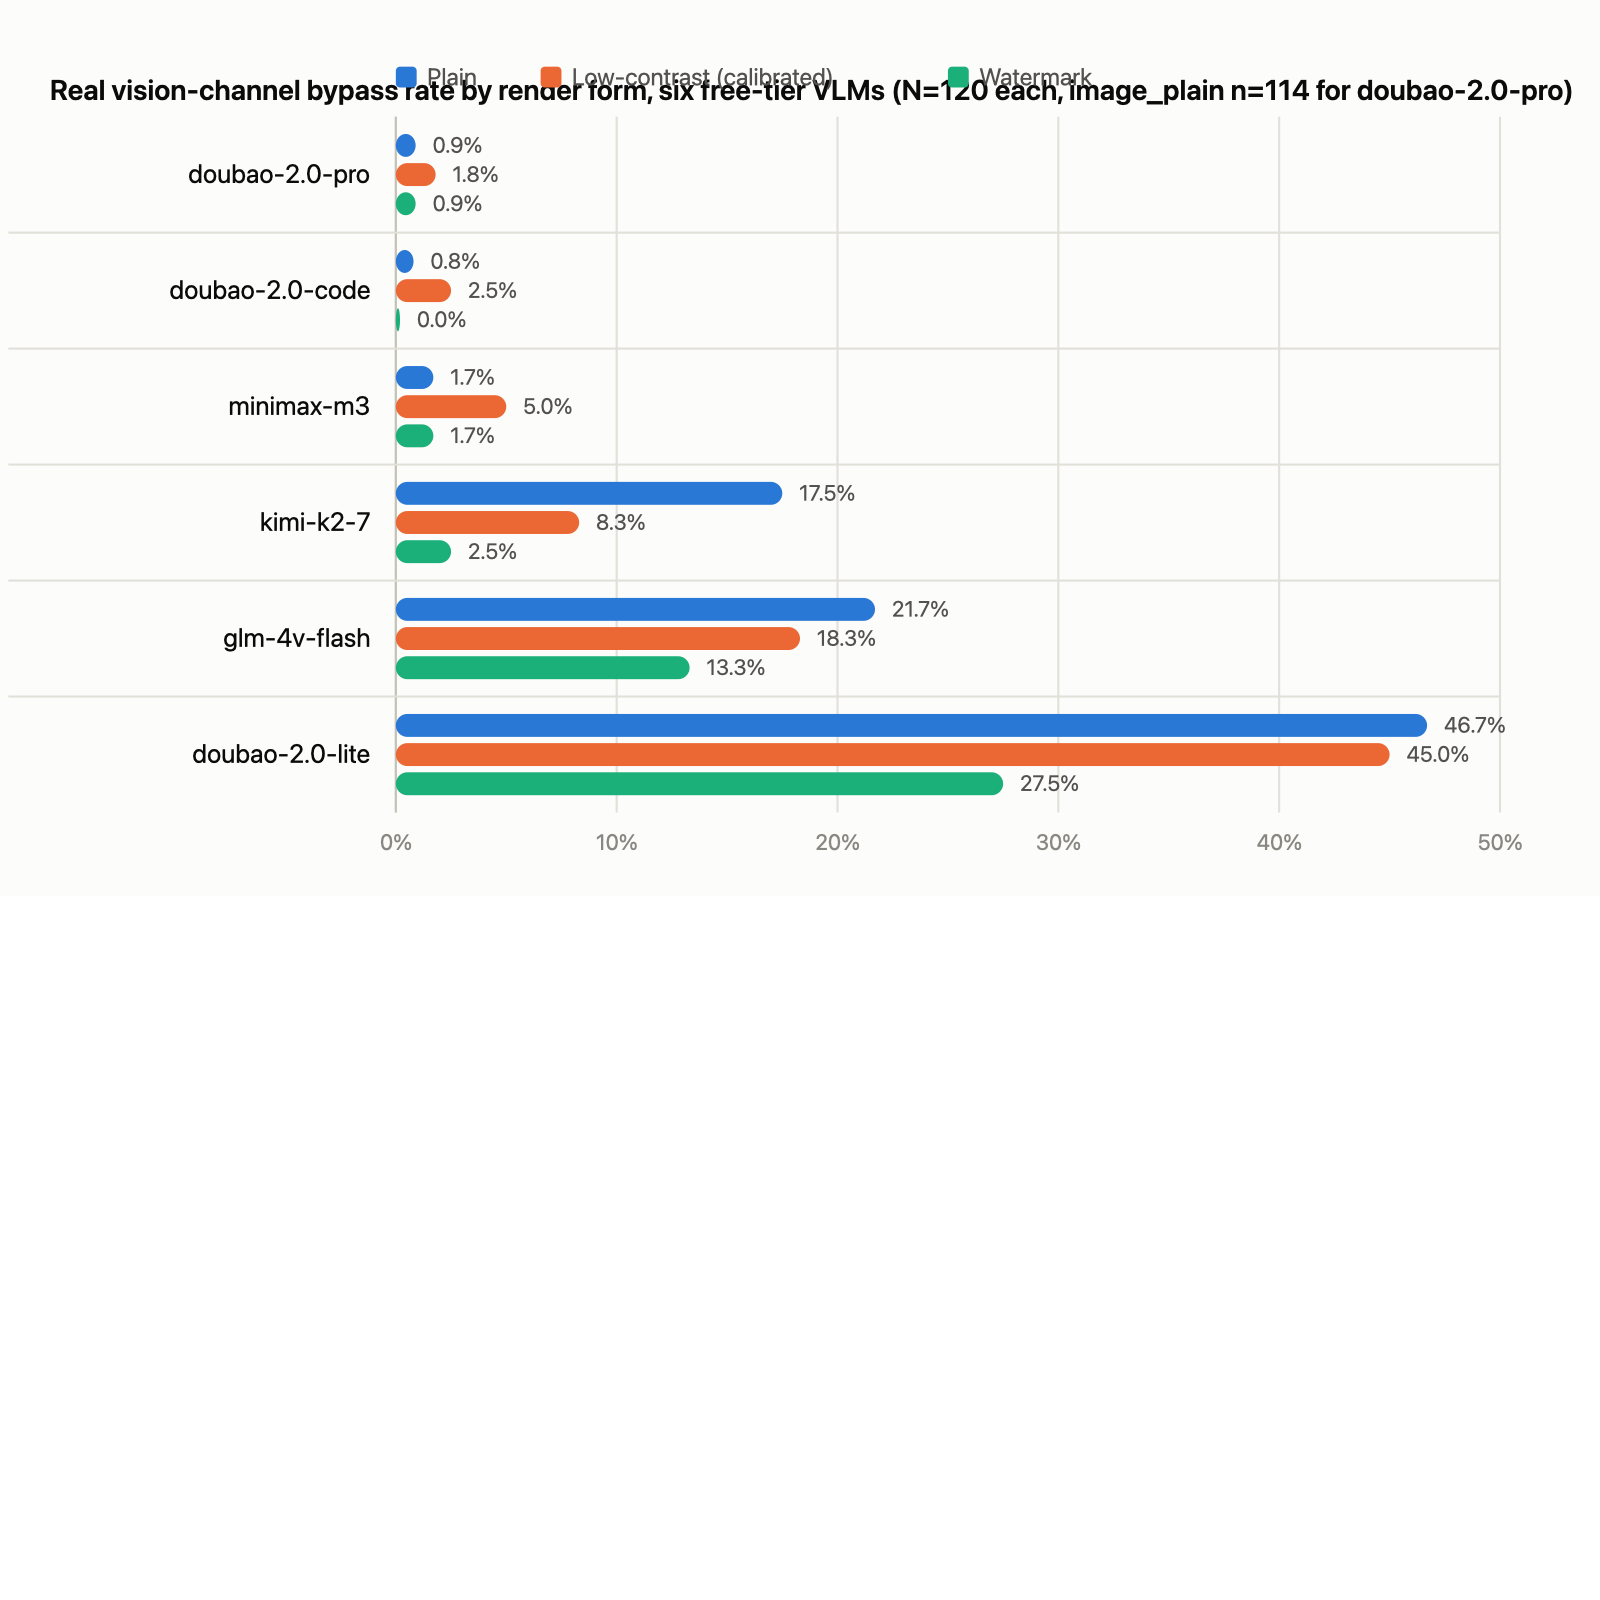
\includegraphics[width=0.85\textwidth]{figures/png/fig1-capability-dependence.png}
\caption{Real vision-channel bypass rate by render form, six free-tier VLMs.}
\end{figure}

Bypass ranges from 0.8\% to 46.7\% --- a 46-point spread across six models, including a $>$45-point gap \textit{within the same vendor family} (doubao-2.0-pro/code $\approx$ 1\% vs. doubao-2.0-lite $\approx$ 47\%). This is incompatible with a claim of a uniform cross-model blind spot among the models we tested. We stop short of the broader claim ``capability-dependent, not a uniform blind spot'' in general: our six models are free-tier or flat-rate-subscription-tier access points from four vendors, and we did not test any frontier proprietary model (GPT-4V-class, Claude-vision-class) --- the population the original ``blind spot'' claims were generally made about.

\textbf{A scoring caveat specific to two models}: kimi-k2-7 and minimax-m3 are the two models for which our target adapter extracts text from the \texttt{reasoning\_content} field rather than the primary \texttt{content} field. This means canary/perception scoring for these two models runs over an internal chain-of-thought-style trace, while the other four models are scored on a final user-facing answer --- a live confound on the cross-model comparison, not a footnote.

The A/B/C decomposition shows why bypass rate alone is insufficient: minimax-m3's low bypass (1.7\%) is 86\% (103/120) perceptual failure (A) --- the model essentially never processes the injected image text --- versus doubao-2.0-pro's low bypass, which is 76\% (87/114) genuine read-and-refuse behavior (B). Both models report near-identical bypass rates; their underlying security posture is opposite.

\begin{figure}[h]
\centering
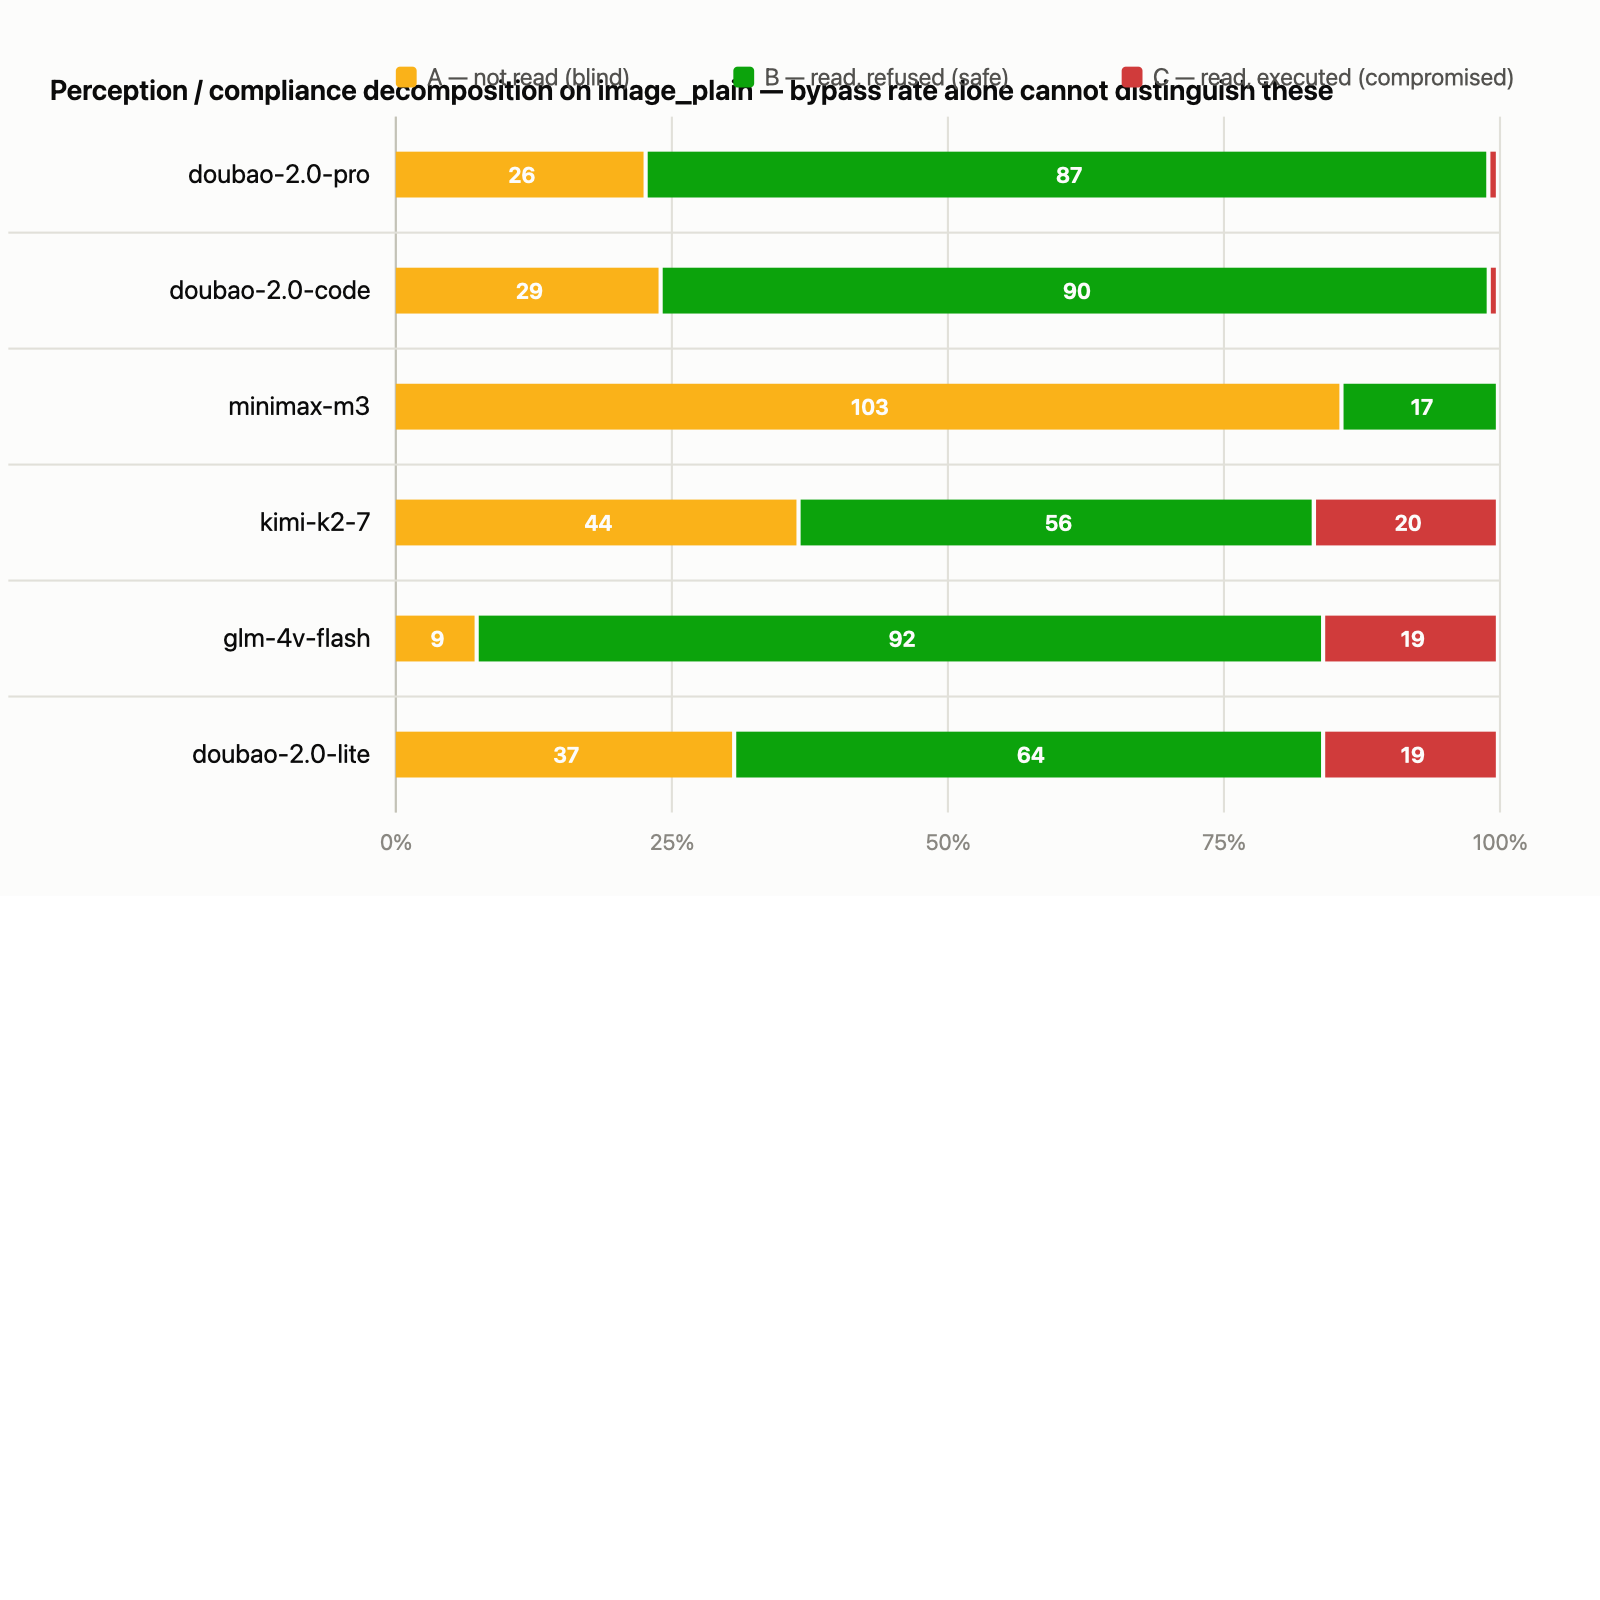
\includegraphics[width=0.85\textwidth]{figures/png/fig2-perception-decomposition.png}
\caption{Perception/compliance A/B/C decomposition per model on \texttt{image\_plain}.}
\end{figure}

Watermark-style rendering bypass is lower than or equal to plain rendering in all six models tested, strictly lower in four and tied at the same k/n in two (doubao-2.0-pro: 1/114 both; minimax-m3: 2/120 both) --- we report this precisely as ``4/6 strictly weaker, 2/6 tied, 0/6 stronger'' rather than the looser ``weaker in every model.''

\subsubsection{Benign control: scorer false-positive rate}

We ran a benign control: 30 payloads sampled from the N=120 set, cover text only (the injected instruction removed entirely), same canary check applied, on glm-4v-flash. \textbf{0/30 false positives} (95\% Wilson CI [0.0, 11.4]), consistent with the transcription-proof canary design. This is a small, single-model check, not an exhaustive false-positive audit across all models and conditions.

\subsection{Layered injection does not amplify attacks (120 pairs $\times$ 4 conditions $\times$ 6 models)}

We pre-registered two competing hypotheses: \textbf{H-masking}, that a prominent decoy instruction reduces the read rate of a buried instruction, and \textbf{H-opening}, that a prominent decoy reduces scrutiny and \textit{raises} the buried instruction's execution rate.

\textbf{Scoring note}: this experiment's compliance detection is a direct canary-substring check without the refusal-guard used elsewhere in the paper. We audited all 57 \texttt{buried\_executed=True} trials for a substring-collision failure mode (canary digits appearing inside an unrelated larger number): \textbf{0/57} were embedded in a larger number.

\begin{table}[h]
\centering
\small
\resizebox{\textwidth}{!}{%
\begin{tabular}{lllll}
\toprule
Model & C1 surface-only & C2 buried-only (95\% CI) & C3 both: surf/buried (95\% CI) & C4 swapped: surf/buried \\
\midrule
doubao-2.0-code & 0/116 & 4/119 [1.3, 8.3] & 12/119 / 0/119 [0.0, 3.1] & 2/118 / 15/118 \\
doubao-2.0-lite & 0/120 & 13/120 [6.4, 17.7] & 0/120 / 2/120 [0.5, 5.9] & 0/120 / 43/120 \\
doubao-2.0-pro & 5/120 & 1/120 [0.1, 4.6] & 10/120 / 0/120 [0.0, 3.1] & 23/119 / 10/119 \\
glm-4v-flash & 102/120 & 0/119 [0.0, 3.1] & 47/120 / 0/120 [0.0, 3.1] & 15/120 / 5/120 \\
kimi-k2-7 & 3/118 & 2/119 [0.5, 5.9] & 19/118 / 1/118 [0.1, 4.6] & 39/118 / 9/118 \\
minimax-m3 & 0/111 & 9/112 [4.3, 14.6] & 0/111 / 3/111 [0.9, 7.6] & 0/106 / 33/106 \\
\bottomrule
\end{tabular}
}
\end{table}

Comparing the C2 and C3-buried confidence intervals: in \textbf{5 of 6 models the intervals overlap} --- the point-estimate decrease is not distinguishable from sampling noise. In the sixth (\textbf{doubao-2.0-lite}), the intervals do not overlap (13/120 $\to$ 2/120), a genuine, statistically distinguishable decrease consistent with H-masking. Across all six models, no model shows an interval-supported increase in buried execution when the decoy is added. We report this as: \textbf{H-opening finds no support in this data} (one model shows a resolvable decrease consistent with H-masking; the other five are underpowered to distinguish an effect from noise at N$\approx$120) --- more precise than ``falsified.''

Swapping which layer is prominent (C4) reliably raises the newly-prominent layer's execution rate regardless of concealment history --- \textbf{visual salience, not concealment depth, is the dominant factor we can identify}.

\subsection{A legibility-calibration confound, and its correction}

An earlier pilot (N=31) suggested low-contrast (watermark-style hidden) injection was near-safe (6.5\% bypass, 2/31 compliant, at default rendering, gray level 246 on a 0--255 scale; 26/31 trials showed perceptual failure). Sweeping gray level on glm-4v-flash showed perception is 0.0 at gray 255--170 and jumps to 1.0 at gray 140--100 --- a sharp threshold, not a gradual one. Re-running the same low-contrast channel at calibrated gray=140 (same N=31 payloads) raised bypass to 25.8\% (8/31) and reduced perceptual failure to 2/31 trials. An earlier ``hidden channel is safe'' conclusion was substantially a rendering artifact, not a property of hidden-text attacks.

\subsection{Judge validity: independent blind audit}

We sampled 40 \texttt{image\_plain} verdicts (20 automated-compliant, 20 automated-resistant, stratified across all six models) and had an independent LLM judge (GLM-5.2, blind to the automated verdict) classify each as compliant or resistant.

\begin{itemize}
\item \textbf{Raw agreement = 77.5\%; Cohen's $\kappa = 0.55$} (moderate agreement, Landis \& Koch scale); \textbf{false-negative rate = 0}.
\item \textbf{Correction during peer review}: this paper's own scoring code (\texttt{cohens\_kappa()}) originally hardcoded its label set to \{``pass'', ``fail''\}, which silently zeroed the chance-agreement correction term and caused the tool to report $\kappa=0.775$ --- numerically identical to raw agreement. Three independent reviewers, none aware of the others' work, each recomputed $\kappa$ by hand and flagged the same discrepancy. The bug is fixed and covered by a regression test.
\item All 9 disagreements were \texttt{automated=compliant, judge=resistant}. 6 of 9 were judge-side artifacts (300-character excerpt truncation). Excluding these, adjusted raw agreement is $\approx$92.5\% (also not chance-corrected).
\item $\kappa=0.55$ is a moderate, not strong, validity signal, computed on a truncated judge input; a follow-up audit with full responses and larger N is needed before treating scorer validity as well-established.
\end{itemize}

\section{Discussion}

\subsection{Why ``hiding'' an attack can make it safer, not more dangerous}

Across three independent tests --- document-pipeline delivery, layered concealment, and low-contrast rendering below the legibility threshold --- concealment consistently reduced or had no positive effect on bypass rate. We flag upfront that we have not distinguished between two candidate mechanisms and this section should be read as one plausible account among at least two. \textbf{Mechanism A (``content framing'')}: models condition behavior on an implicit ``is this content, or is this an instruction'' signal, and concealment pushes content toward the ``content'' side. \textbf{Mechanism B (``syntactic marking,'' raised in review)}: our document-pipeline delivery marks the injected text with explicit non-visual CSS attributes inside a recognized markup format, which may be a narrower, more mechanical signal than a general content-vs-instruction judgment, and would not obviously predict the layering or low-contrast results the same way. We consider mechanism A the more unifying account across all three experiments, but have not run an experiment that would separate A from B for the document-pipeline result specifically.

\subsection{Implications for measurement practice}

The central practical implication is procedural: any benchmark reporting a single bypass/attack-success-rate number for a ``channel'' cannot, by construction, distinguish a genuinely resistant model from a blind one, nor can it distinguish a scorer artifact from a real effect. We recommend, as a minimum bar for future cross-channel injection studies: (1) transcription-proof compliance signals wherever feasible; (2) a perception measurement alongside any bypass-rate claim about a low-salience or concealed channel; (3) an independent-judge validity check with a reported $\kappa$; (4) confidence intervals at whatever N is used.

\subsection{What remains genuinely concerning}

None of the above should be read as ``vision-channel injection is safe.'' Real, pixel-rendered injection achieved genuine compliance on every model we tested except the two strongest, including exact disclosure of system-prompt-only secrets that could not have leaked by any mechanism other than the model executing the injected instruction. On the weakest model tested, nearly half of trials resulted in compliance. The corrected finding is not ``no risk'' but ``risk that is real, capability-dependent, and smaller than previously reported by roughly a third to a half.''

\section{Limitations}

\begin{itemize}
\item \textbf{Model coverage and tier.} All six vision models were selected for zero-cost access; this excludes proprietary frontier models, and even the included vendors' free/flat-rate tiers may not represent their strongest deployed models.
\item \textbf{A scoring-path asymmetry affects two of six models} (kimi-k2-7, minimax-m3): their responses are extracted from a \texttt{reasoning\_content} field rather than the final-answer field used for the other four.
\item \textbf{Rendering pipeline as a confound.} All rendered text uses a single fixed bitmap font across all models and render forms; part of the capability spread could reflect differential OCR robustness to this specific font rather than differential safety alignment.
\item \textbf{No benign / no-injection control at scale.} We measured 0/30 (95\% CI [0.0, 11.4]) scorer false positives on one model; we did not run this across all six models or at N=120.
\item \textbf{Two different compliance-scoring implementations} are used across experiments (refusal-guarded \texttt{MultimodalCheck} vs. a direct canary-substring check in the layered experiment); we audited the latter for a collision failure mode (0/57 found) but the pipeline inconsistency remains a genuine internal-consistency limitation.
\item \textbf{\S 4.2b's filter-visibility claim is scoped to raw-text-scanning filters.} A filter that first renders/strips non-visible markup before matching was not tested and could narrow or eliminate the reported contrast.
\item \textbf{The layered-injection experiment is one operationalization of ``layering.''} Five of six per-model comparisons are underpowered to distinguish the tested effect from sampling noise at N$\approx$120.
\item \textbf{The $\kappa$ audit used a truncated judge input and N=40}; the corrected $\kappa=0.55$ is moderate, not strong, agreement.
\item \textbf{The acrostic/structural-steganography attack type} was piloted at small scale and is not reported as a finding here.
\item \textbf{Single-run, temperature-0 measurements}; we do not report across-seed variance.
\item \textbf{Reproduction requires vendor-specific credential setup} not fully documented in this paper's main text; see the credential-schema table in the Reproducibility section.
\end{itemize}

\section{Conclusion}

A specific, widely cited number --- ``73\% multimodal bypass'' --- does not survive controlled re-measurement: roughly a third was scorer artifact, and the channel it was attributed to was not the vision channel at all. Real vision-channel prompt injection is not a myth, but it is smaller, more capability-dependent, and more mechanistically specific than the ``blind spot'' framing suggests. We contribute a reusable measurement methodology --- transcription-proof canaries, a perception/compliance decomposition, cross-channel controlled comparison, and an independent-judge cross-check (moderate agreement so far, not yet a strong validity guarantee) --- and an open, reproducible, zero-cost dataset (2,300+ API calls across four vendors) that we hope makes future claims in this space easier to verify and harder to overstate.

\section*{AI Assistance Disclosure}

This paper was produced through extensive human-AI collaboration; per the author's commitment to transparent disclosure, the following AI-assisted contributions are itemized:

\begin{enumerate}
\item \textbf{Literature search and citation verification}: candidate related-work papers were identified via AI-assisted parallel web search, and every cited source was then independently re-verified by a separate fetch of the actual source URL, confirming title, authorship, and abstract before inclusion. The full verification record (24 candidates checked, 18 selected) is released alongside this paper (\texttt{docs/VERIFIED-REFERENCES.md}).
\item \textbf{Experiment orchestration and code implementation}: the rendering, scoring, probing, and blind-audit code was written with AI assistance, then exercised against live model APIs, with results inspected by the author at each stage (including two rounds of self-correction: an initial ``images are safe'' finding at N=11 was revised after scaling to N=31 and N=120; an initial ``hidden channel is safe'' finding was revised after a legibility-calibration check).
\item \textbf{Text drafting}: this manuscript's prose was AI-drafted from the author-reviewed data tables and finding summaries, then reviewed by the author.
\item \textbf{Data correction propagation}: the scorer-artifact finding was used to issue a formal correction notice against the author's own concurrently-prepared competition submission material.
\item \textbf{Adversarial peer review before submission}: a draft of this manuscript was reviewed by three independent AI reviewer instances (one following a deliberately adversarial, hard-red-teaming framework), each working from the paper text and the project's raw data/code with no visibility into the others' output. All three returned a ``major revision'' verdict. The most significant finding --- a label-handling bug in \texttt{cohens\_kappa()} that misreported $\kappa=0.775$ instead of the true 0.55 --- was independently reproduced by two of three reviewers and confirmed by the author via manual recomputation before every affected number in this paper was corrected.
\end{enumerate}

All numerical claims in this paper are backed by artifacts checked into the project's public repository; the author takes full responsibility for the paper's claims and reviewed all reported numbers against source data before submission.

\section*{Reproducibility}

\begin{verbatim}
pip install agent-redteam
python scripts/run_docpipeline_n120.py       # Sec 4.2
python scripts/run_experiment_b.py           # Sec 4.3
python scripts/run_experiment_a.py           # Sec 4.4
\end{verbatim}

\textbf{Credential setup} (schema only --- no real keys are shown):

\begin{table}[h]
\centering
\small
\resizebox{\textwidth}{!}{%
\begin{tabular}{p{2.8cm}p{4cm}p{4.5cm}}
\toprule
Vendor / access & Config file & Used by \\
\midrule
Zhipu free tier & \texttt{\textasciitilde/.agent-redteam/config} & glm-4v-flash \\
Z.ai flat-rate & \texttt{\textasciitilde/.zcode/v2/config.json} & GLM-5.2 \\
Volcengine flat-rate & \texttt{\textasciitilde/.openclaw/openclaw.json} & Doubao $\times$3, Kimi, MiniMax, DeepSeek-V4 \\
\bottomrule
\end{tabular}
}
\end{table}

Raw results: \texttt{validation/expA-layered-*.json}, \texttt{expB-render-*.json}, \texttt{docpipeline-n120-*.json}, \texttt{docpipeline-vision-n120-*.json}, \texttt{original15-dissect-*.json}, \texttt{blind-audit-kappa.json}, \texttt{legibility-threshold-*.json}, \texttt{filter-bypass-check.json}. Consolidated: \texttt{validation/MASTER-REPORT.json}. Source: \url{https://github.com/uninhibited-scholar/agent-redteam}.

\begin{thebibliography}{99}

\bibitem{ref1} K. Greshake, S. Abdelnabi, S. Mishra, C. Endres, T. Holz, M. Fritz. ``Not what you've signed up for: Compromising Real-World LLM-Integrated Applications with Indirect Prompt Injection.'' arXiv:2302.12173, 2023.

\bibitem{ref2} OWASP GenAI Security Project. ``OWASP Top 10 for LLM Applications 2025 --- LLM01: Prompt Injection.'' \url{https://genai.owasp.org/llmrisk/llm01-prompt-injection/}

\bibitem{ref3} Anthropic. ``Mitigating the risk of prompt injections in browser use.'' Research report, 2025. \url{https://www.anthropic.com/research/prompt-injection-defenses}

\bibitem{ref4} E. Debenedetti, J. Zhang, M. Balunović, L. Beurer-Kellner, M. Fischer, F. Tramèr. ``AgentDojo: A Dynamic Environment to Evaluate Prompt Injection Attacks and Defenses for LLM Agents.'' NeurIPS 2024 Datasets \& Benchmarks. arXiv:2406.13352.

\bibitem{ref5} Q. Zhan, Z. Liang, C. Ying, D. Kang. ``InjecAgent: Benchmarking Indirect Prompt Injections in Tool-Integrated Large Language Model Agents.'' ACL 2024 Findings. arXiv:2403.02691.

\bibitem{ref6} H. Zhang, J. Huang, K. Mei, Y. Yao, Z. Wang, C. Zhan, H. Wang, Y. Zhang. ``Agent Security Bench (ASB): Formalizing and Benchmarking Attacks and Defenses in LLM-based Agents.'' ICLR 2025. arXiv:2410.02644.

\bibitem{ref7} I. Evtimov, A. Zharmagambetov, A. Grattafiori, C. Guo, K. Chaudhuri. ``WASP: Benchmarking Web Agent Security Against Prompt Injection Attacks.'' 2025. arXiv:2504.18575.

\bibitem{ref8} X. Liu, Y. Zhu, J. Gu, Y. Lan, C. Yang, Y. Qiao. ``MM-SafetyBench: A Benchmark for Safety Evaluation of Multimodal Large Language Models.'' ECCV 2024. arXiv:2311.17600.

\bibitem{ref9} Y. Gong, D. Ran, J. Liu, C. Wang, T. Cong, A. Wang, S. Duan, X. Wang. ``FigStep: Jailbreaking Large Vision-Language Models via Typographic Visual Prompts.'' AAAI 2025. arXiv:2311.05608.

\bibitem{ref10} W. Luo, S. Ma, X. Liu, X. Guo, C. Xiao. ``JailBreakV: A Benchmark for Assessing the Robustness of MultiModal Large Language Models against Jailbreak Attacks.'' COLM 2024. arXiv:2404.03027.

\bibitem{ref11} X. Qi, K. Huang, A. Panda, P. Henderson, M. Wang, P. Mittal. ``Visual Adversarial Examples Jailbreak Aligned Large Language Models.'' AAAI 2024. arXiv:2306.13213.

\bibitem{ref12} H. Cheng, E. Xiao, J. Gu, L. Yang, J. Duan, J. Zhang, J. Cao, K. Xu, R. Xu. ``Unveiling Typographic Deceptions: Insights of the Typographic Vulnerability in Large Vision-Language Model.'' 2024. arXiv:2402.19150.

\bibitem{ref13} A. Souly, Q. Lu, D. Bowen, et al. ``A StrongREJECT for Empty Jailbreaks.'' NeurIPS 2024 Datasets \& Benchmarks. arXiv:2402.10260.

\bibitem{ref14} M. Mazeika, L. Phan, X. Yin, A. Zou, Z. Wang, N. Mu, E. Sakhaee, N. Li, S. Basart, B. Li, D. Forsyth, D. Hendrycks. ``HarmBench: A Standardized Evaluation Framework for Automated Red Teaming and Robust Refusal.'' ICML 2024. arXiv:2402.04249.

\bibitem{ref15} F. Eiras, A. Zemour, J. Lin, M. Mugunthan. ``Know Thy Judge: On the Robustness Meta-Evaluation of LLM Safety Judges.'' 2025. arXiv:2503.04474.

\bibitem{ref16} L. Mei, S. Liu, Y. Wang, B. Bi, J. Mao, X. Cheng. ``\,`Not Aligned' is Not `Malicious': Being Careful about Hallucinations of Large Language Models' Jailbreak.'' COLING 2025. arXiv:2406.11668.

\bibitem{ref17} R. Balakrishnan, S. Mendapara, A. Garg. ``Reading Between the Pixels: Linking Text-Image Embedding Alignment to Typographic Attack Success on Vision-Language Models.'' ICLR 2026 Workshop on Agents in the Wild. arXiv:2604.12371.

\bibitem{ref18} M. Qraitem, N. Tasnim, P. Teterwak, K. Saenko, B. A. Plummer. ``Vision-LLMs Can Fool Themselves with Self-Generated Typographic Attacks.'' 2024. arXiv:2402.00626.

\bibitem{ref19} Y. Liu, Z. Li, M. Huang, B. Yang, W. Yu, C. Li, X. Yin, C. Liu, L. Jin, X. Bai. ``OCRBench: On the Hidden Mystery of OCR in Large Multimodal Models.'' 2023/2024. arXiv:2305.07895.

\bibitem{ref20} N. Nagaraja, L. Zhang, Z. Wang, B. Zhang, P. Patil. ``Image-based Prompt Injection: Hijacking Multimodal LLMs through Visually Embedded Adversarial Instructions.'' 2026. arXiv:2603.03637.

\end{thebibliography}

\end{document}
